% !TEX root = 1_power_supply.tex
\documentclass[1_power_supply.tex]{subfiles}
\graphicspath{{../figures/}}
\begin{document}

\section{DC-DCコンバータ}

  \subsection{目的}

    太陽電池から得られる直流の電圧,電流を増幅するためにDC-DCコンバータのうち,チュックコンバータを用いる.本実験では,チュックコンバータのスイッチ制御を変化させたときの電力利得を調べる.

  \subsection{原理}

    DC-DCコンバータは,スイッチングを行うことで電圧を増幅できる装置である.1周期のスイッチングの中でのオンの時間の割合(デューティ比 $D$)によって,入力電圧$V_\mathrm{i}$と出力電圧$V_\mathrm{o}$との間に
    \begin{align}
      V_\mathrm{o} = -\frac{D}{1-D}V_\mathrm{i}
    \end{align}

    という関係が成り立つ.

  \subsection{方法}


    \begin{figure}[htbp]
      \begin{center}
        \scalebox{0.1}{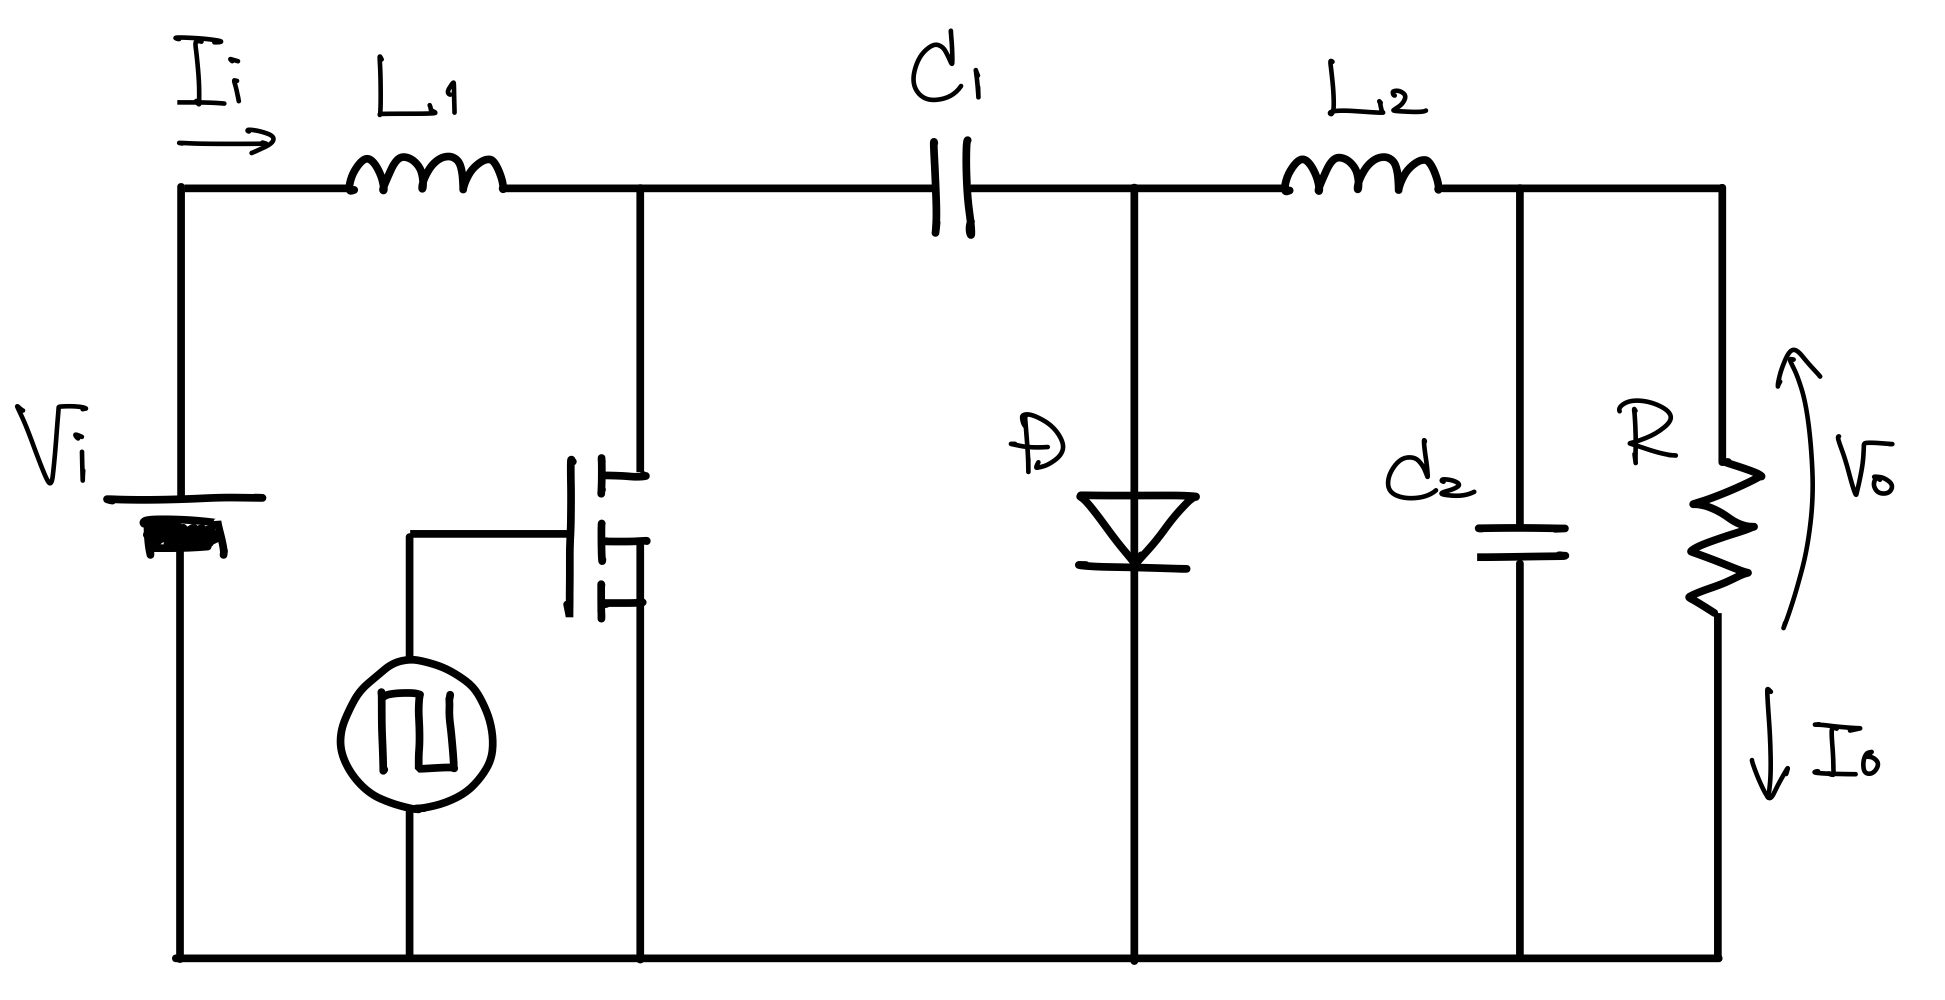
\includegraphics{1_4.png}}
        \caption{測定対象の回路}\label{fig:1_4}
      \end{center}
    \end{figure}

    測定対象の回路を図\ref{fig:1_4}に示す.この回路に対して,方形波でデューティ比がそれぞれ \\$\SIs{10}{\percent},\SIs{25}{\percent},\SIs{40}{\percent},\SIs{50}{\percent},\SIs{60}{\percent},\SIs{75}{\percent},\SIs{80}{\percent}$のものを印加したときの入力電圧$V_\mathrm{i}$,入力電流$I_\mathrm{i}$,出力電圧$V_\mathrm{o}$,出力電流$I_\mathrm{o}$を測定し,入力電力$P_\mathrm{i}$と出力電力$P_\mathrm{o}$の関係をプロットする.
    各素子や信号の詳細は,
    \begin{enumerate}
      \item $L_1=\SIs{470}{\text{\textmu}\henry}$ % \micro が使えなかったのでやむを得ず
      \item $L_2=\SIs{470}{\text{\textmu}\henry}$
      \item $C_1=\SIs{100}{\text{\textmu}\farad}$
      \item $C_2=\SIs{100}{\text{\textmu}\farad}$
      \item 方形波 : (周波数 : $\SIs{100}{kHz}$, 電圧 : $\SIs{5}{\vpp}$, オフセット : $\SIs{2.5}{\volt}$)
    \end{enumerate}
    である.

  \subsection{使用器具}

    (型番については確認し次第追記します.)
    \begin{enumerate}
      \item 電圧計
      \item 電流計
      \item 直流電源
      \item ファンクションジェネレータ
    \end{enumerate}

  \subsection{結果}

    各デューティ比$D$での電力利得を図\ref{fig:2_10p},\ref{fig:2_25p},\ref{fig:2_40p},\ref{fig:2_50p},\ref{fig:2_60p},\ref{fig:2_75p},\ref{fig:2_80p},に示す.


    \begin{figure}[htbp]
      \begin{minipage}{0.45\columnwidth}
        \centering
        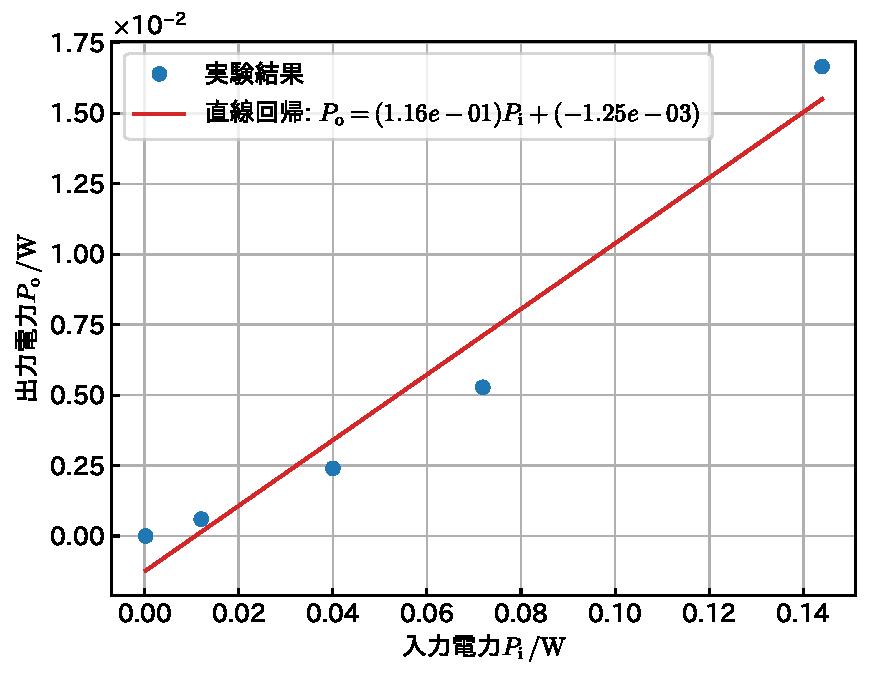
\includegraphics[width=0.8\columnwidth]{2_10p.pdf}
        \caption{$D=0.1$}\label{fig:2_10p}
      \end{minipage}
      \begin{minipage}{0.45\columnwidth}
        \centering
        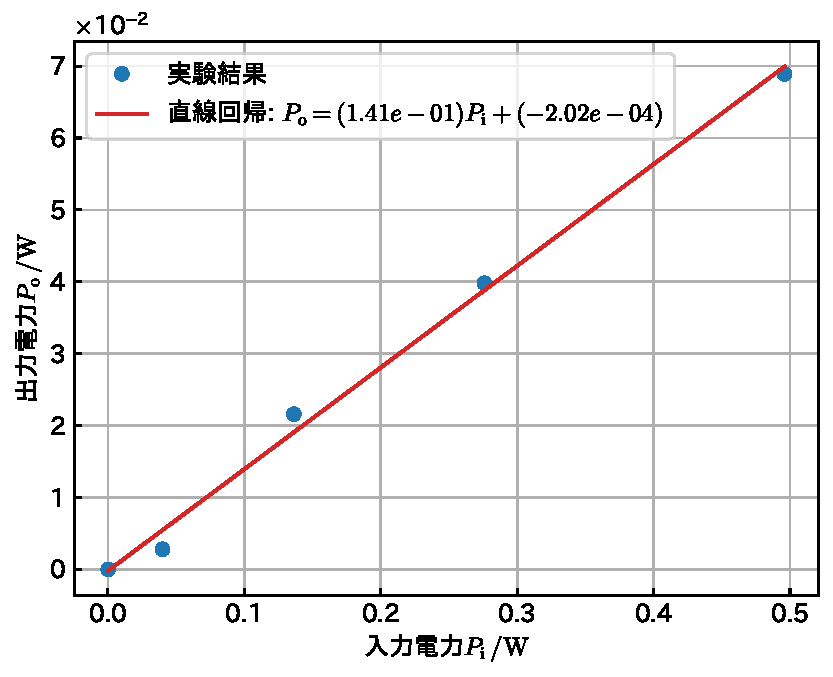
\includegraphics[width=0.8\columnwidth]{2_25p.pdf}
        \caption{$D=0.25$}\label{fig:2_25p}
      \end{minipage}

      \vspace{1.5mm}
      \begin{minipage}{0.45\columnwidth}
        \centering
        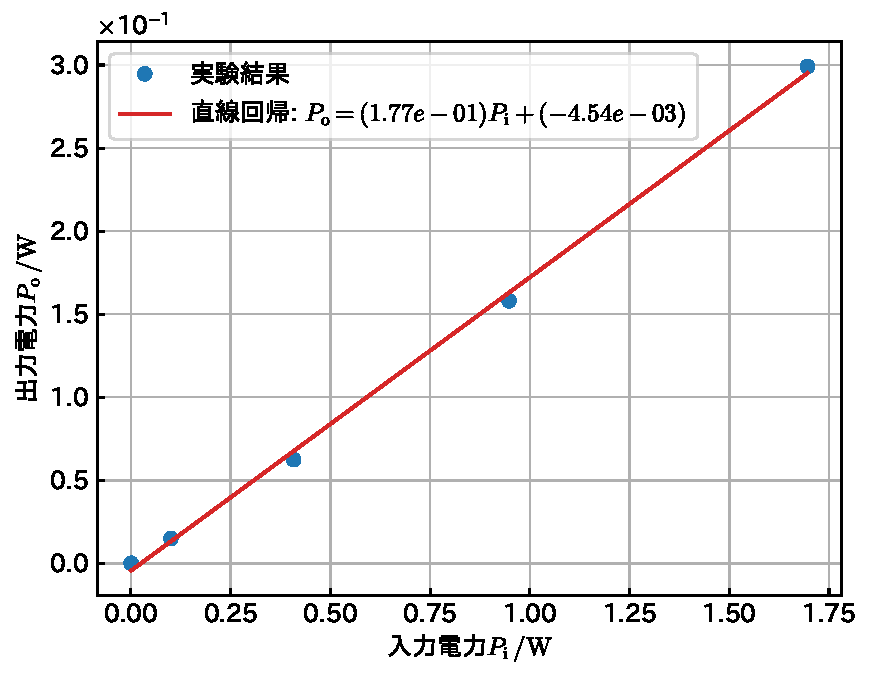
\includegraphics[width=0.8\columnwidth]{2_40p.pdf}
        \caption{$D=0.4$}\label{fig:2_40p}
      \end{minipage}
      \begin{minipage}{0.45\columnwidth}
        \centering
        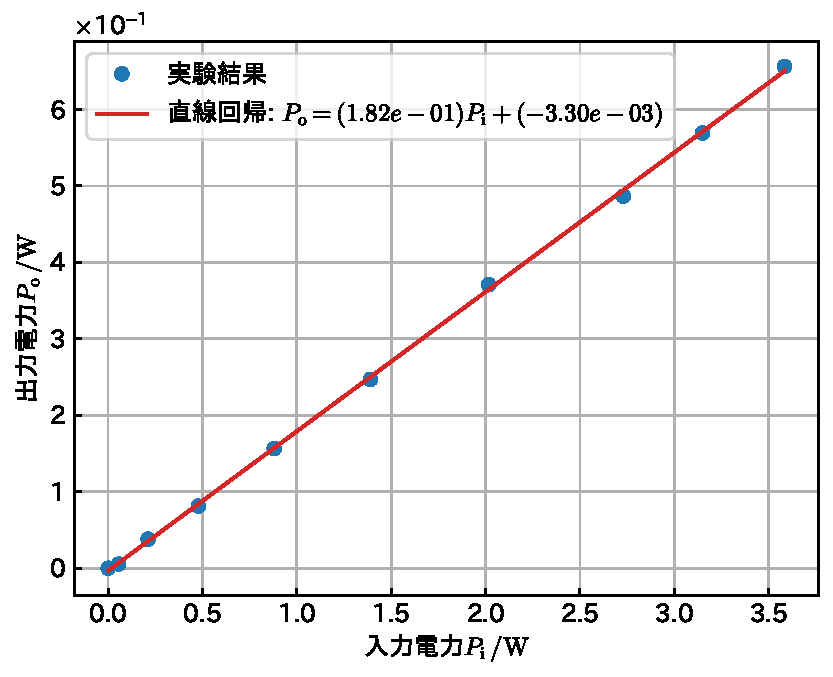
\includegraphics[width=0.8\columnwidth]{2_50p.pdf}
        \caption{$D=0.5$}\label{fig:2_50p}
      \end{minipage}

      \vspace{1.5mm}
      \begin{minipage}{0.45\columnwidth}
        \centering
        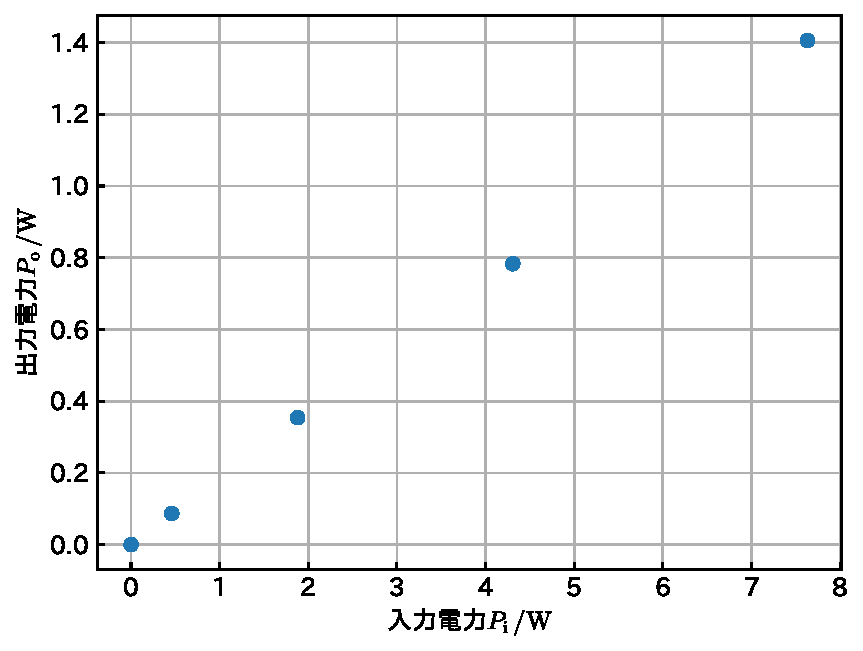
\includegraphics[width=0.8\columnwidth]{2_60p.pdf}
        \caption{$D=0.6$}\label{fig:2_60p}
      \end{minipage}
      \begin{minipage}{0.45\columnwidth}
        \centering
        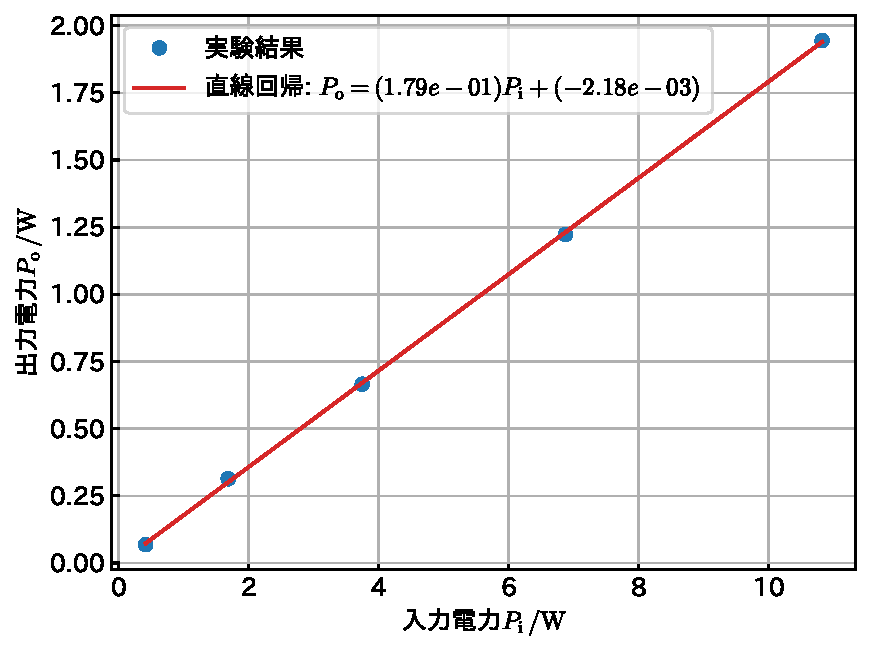
\includegraphics[width=0.8\columnwidth]{2_75p.pdf}
        \caption{$D=0.75$}\label{fig:2_75p}
      \end{minipage}

      \vspace{1.5mm}
      \begin{minipage}{0.45\columnwidth}
        \centering
        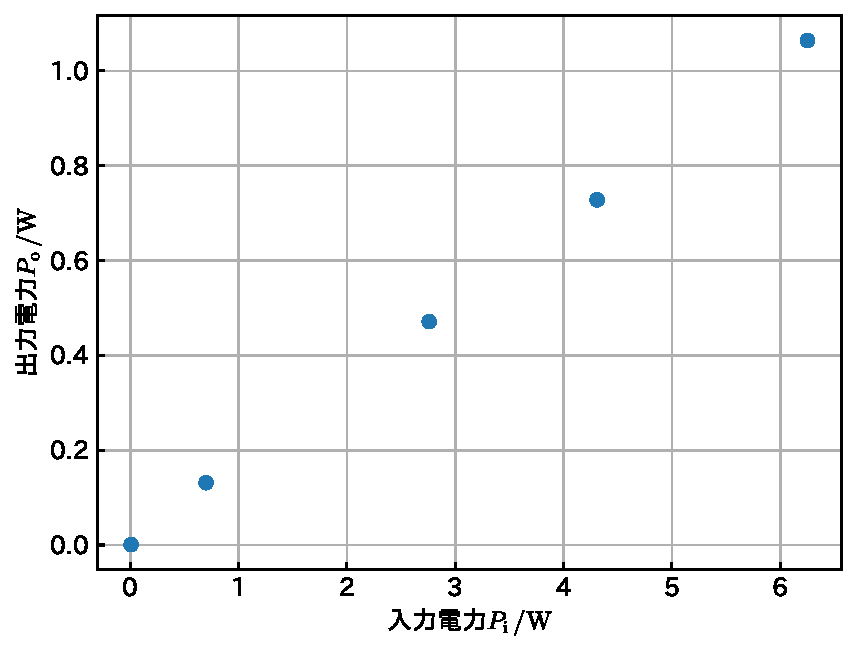
\includegraphics[width=0.8\columnwidth]{2_80p.pdf}
        \caption{$D=0.8$}\label{fig:2_80p}
      \end{minipage}
      \begin{minipage}{0.45\columnwidth}
        \centering
        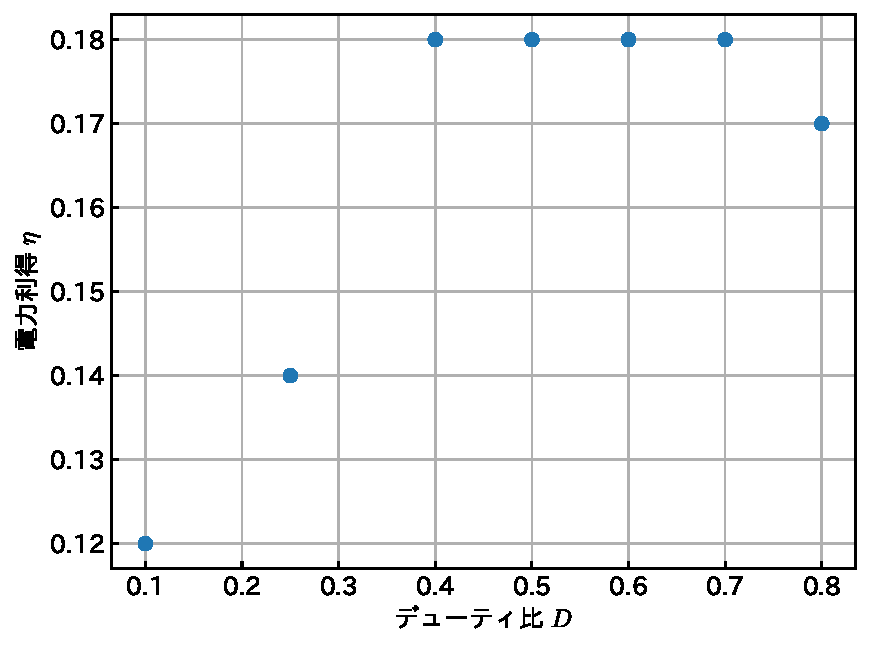
\includegraphics[width=0.8\columnwidth]{2_d_eta.pdf}
        \caption{デューティ比と電力利得の関係}\label{fig:2_d_eta}
      \end{minipage}
    \end{figure}

  \subsection{考察}

    デューティ比と電力利得の関係を表すプロットを図\ref{fig:2_d_eta}に示す.この関係から,電力利得を良くするためにはデューティ比が$0.4\sim 0.7$の範囲で動作させればいいことがわかる.

\end{document}
